\subsection{Einführung}
\begin{frame}
\frametitle{Was ist Apache Kafka?}
\begin{columns}[T]
	\begin{column}[T]{0.49\textwidth}
		
	\end{column}
	\begin{column}[T]{0.49\textwidth}
		
\end{column}
\end{columns}
	\centering
	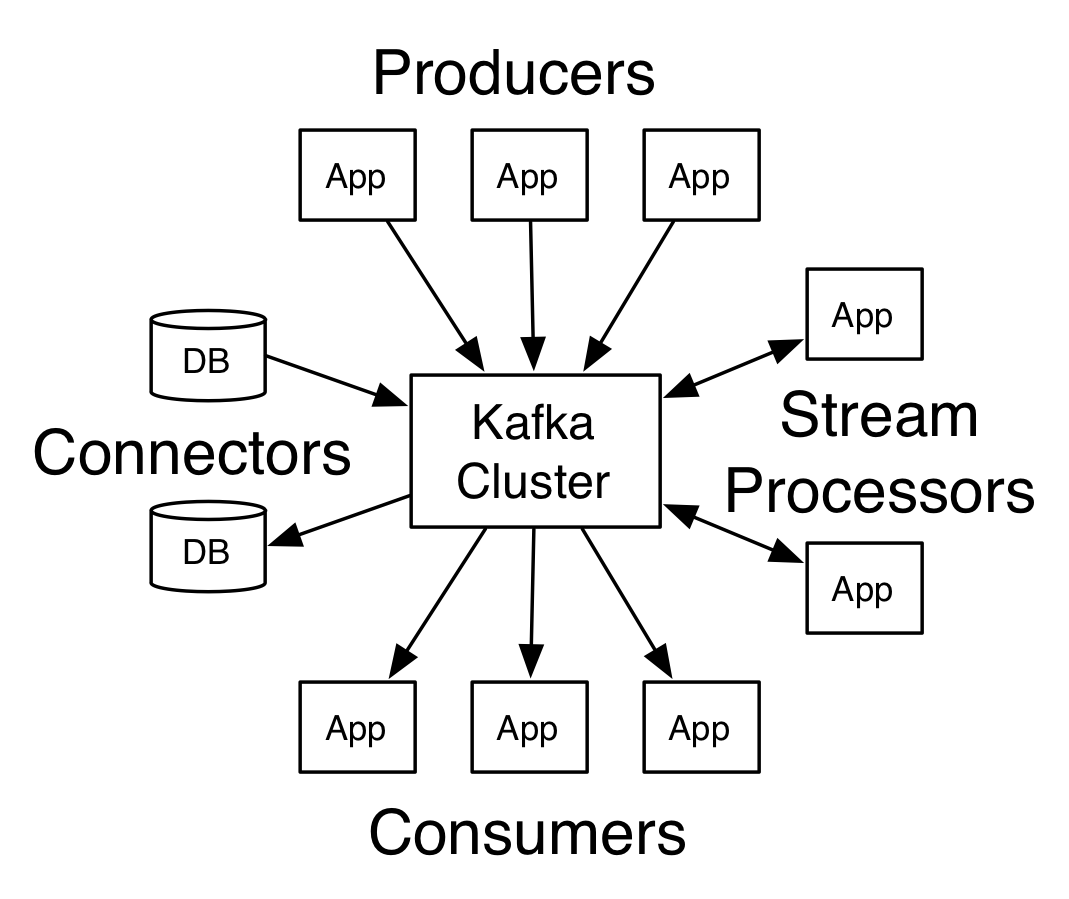
\includegraphics[scale=1.2]{figure/kafka-apis.png}

	Apache Kafka ist eine verteilte skalierbare Streaming Plattform.

	\BottomRightText{\textit{Graphics based on}~\cite{Kafka}}

	\pnote{* APIs sind hier abgebildet.}
\end{frame}

\begin{frame}{Motivation}
\begin{figure}
	\centering
	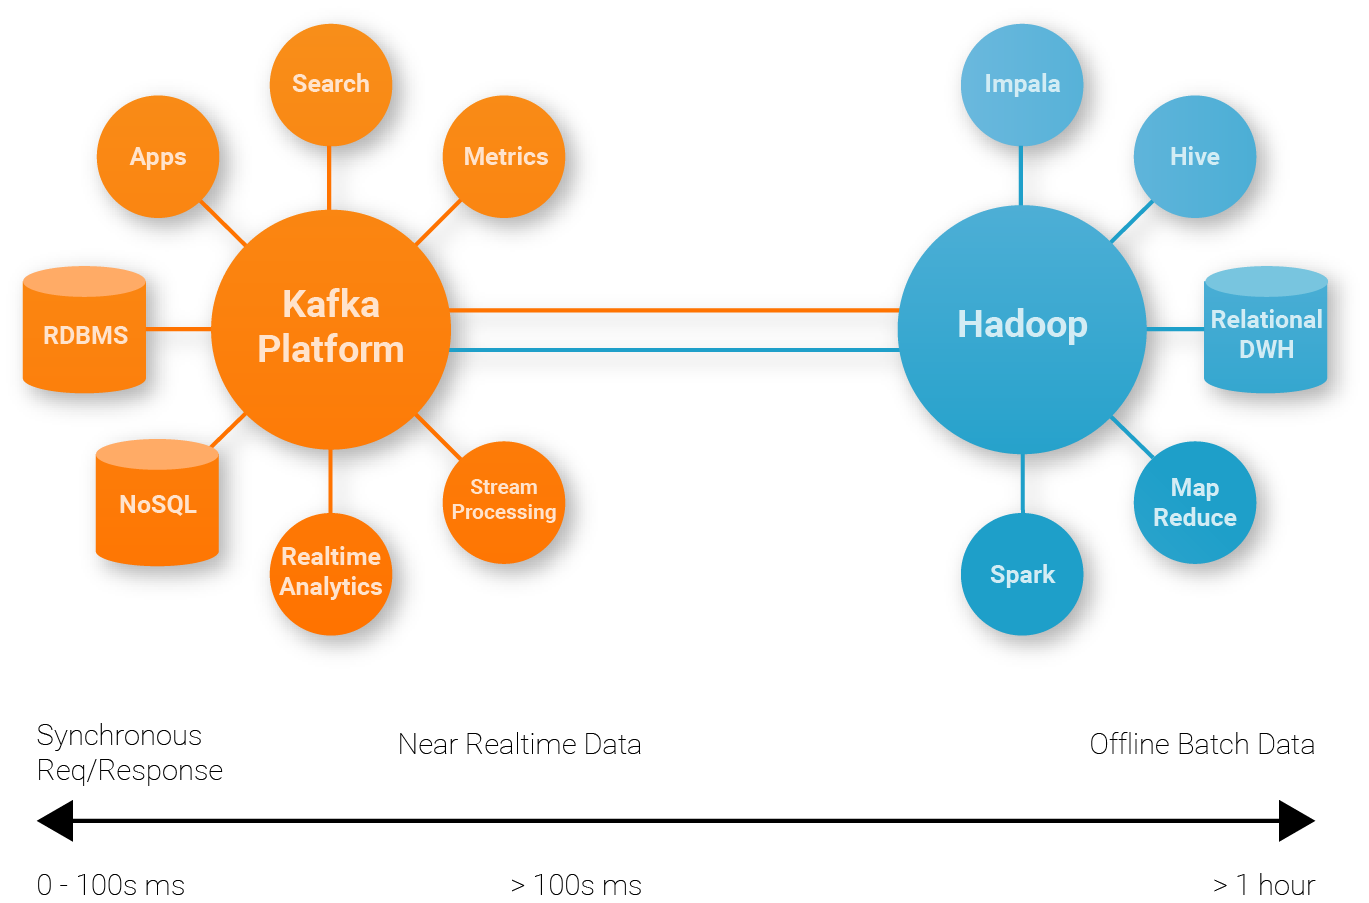
\includegraphics[scale=0.165]{figure/kafka_vs_hadoop.png}
	\caption{Kafka and Hadoop~\cite{Rao17}}
\end{figure}
\end{frame}

\begin{frame}
\frametitle{Eigenschaften}
Kafka ...
\begin{itemize}
	\item ist ein Message Queuing System
	\item kann Nachrichten speichern
	\item kann Nachrichten verarbeiten
	\item kann all das in Echtzeit
\end{itemize}

\end{frame}

\begin{frame}
\frametitle{Unternehmen und Use Cases}

\begin{tabular}{cl}
	\raisebox{-.25\height}{
\includegraphics[scale=0.2]{figure/linkedin_logo.pdf}} 
		& Operational Metrics\\~\\
	\raisebox{-.25\height}{
\includegraphics[scale=0.2]{figure/cisco_logo.pdf}} 
		& OpenSOC (Security Operations Center)\\~\\
	\raisebox{-.25\height}{
\includegraphics[scale=0.08]{figure/netflix_logo.pdf}} 
		& Real-time Monitoring and Event-processing Pipeline\\~\\
	\raisebox{-.25\height}{
\includegraphics[scale=0.2]{figure/spotify_logo.pdf}} 
		& Log Delivery System\\~\\
	\raisebox{-.25\height}{
\includegraphics[scale=0.1]{figure/twitter_logo.pdf}} 
		& Part of Storm Stream Processing Infrastructure
		
		\pnote{* Messaging, Website Activity Tracking, Metriken, Log Verarbeitung, Datenstromverarbeitung}
		
		\pnote{* Zentrale Data Pipeline }
		\pnote{- 1.4 Billarden Narichten/Tag 1400 Broker} % https://engineering.linkedin.com/blog/2016/04/kafka-ecosystem-at-linkedin
		\pnote{* OpenSecurityOperationsCenter}
		\pnote{- Als Messaging System zwischen Data Collection und Real Time Processing}
		% We currently operate 36 Kafka clusters consisting of 4,000+ broker instances for both Fronting Kafka and Consumer Kafka. More than 700 billion messages are ingested on an average day.
		\pnote{- Zum Einsammeln von Clientdaten eingesetzt}
		
\end{tabular}
\end{frame}


\subsection{Grundlagen (Queue \& Topic)}

%% Was sind Records? -> Auf Folie aufnehmen.

\begin{frame}
\frametitle{Queue}
	\begin{center}
		\centering
		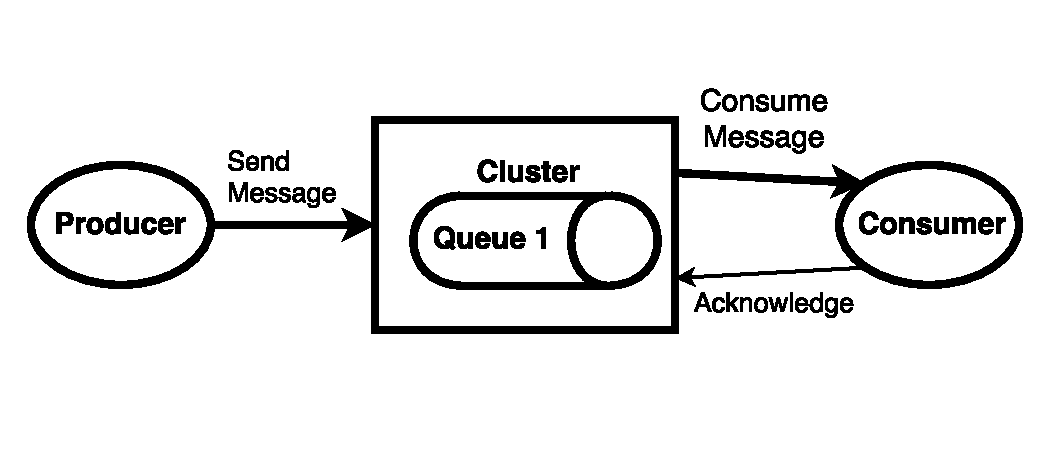
\includegraphics[scale=0.6]{figure/queue_draw.pdf}
	\end{center}
	
	\BottomRightText{\textit{Graphics based on}~\cite{Bengel14}}
\end{frame}

\begin{frame}
\frametitle{Topic}
	\centering
	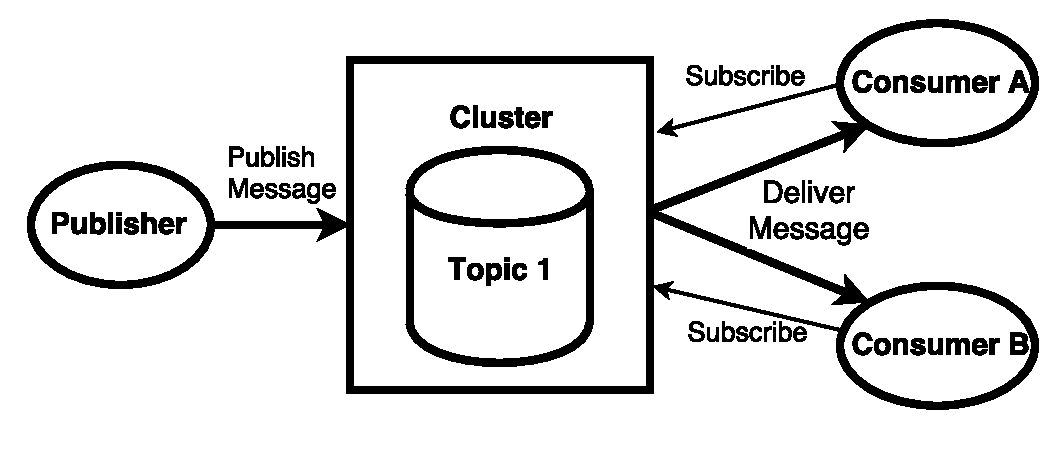
\includegraphics[scale=0.6]{figure/topic_draw.pdf}
	
	\BottomRightText{\textit{Graphics based on}~\cite{Bengel14}}
\end{frame}

%% Messaging System
\begin{frame}
\frametitle{Zusammenfassung}

Bisher: 
\begin{itemize}
	\item Queueing
	\begin{itemize}
		\item Nachricht 1:1 Consumer
		\item Nachrichtenverarbeitung skaliert
		\item Nachricht kann nur einmal abgerufen werden
	\end{itemize}
	\item Topic
	\begin{itemize}
		\item Nachrichten 1:N Consumer
		\item Nachrichten werden verteilt
		\item Skaliert nicht  			%Jeder bekommt die Nachricht. Daher nicht horizontal skallierbar.
	\end{itemize}
\end{itemize}
\end{frame}

\subsection{Kafka Topic}
\begin{frame}
\frametitle{Kafka Topic}
\centering
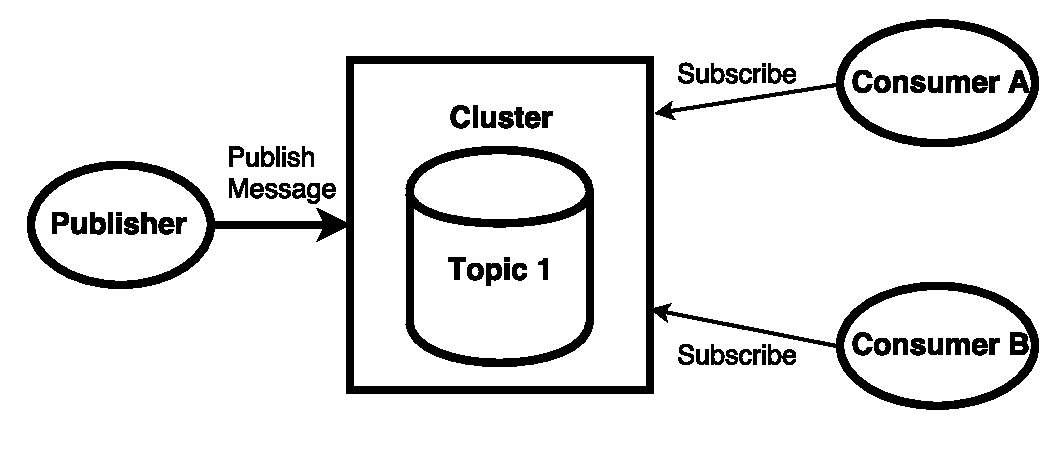
\includegraphics[scale=0.6]{figure/Kafka_topic_draw_subscribe.pdf}
\end{frame}

\begin{frame}
\frametitle{Kafka Topic}
\centering
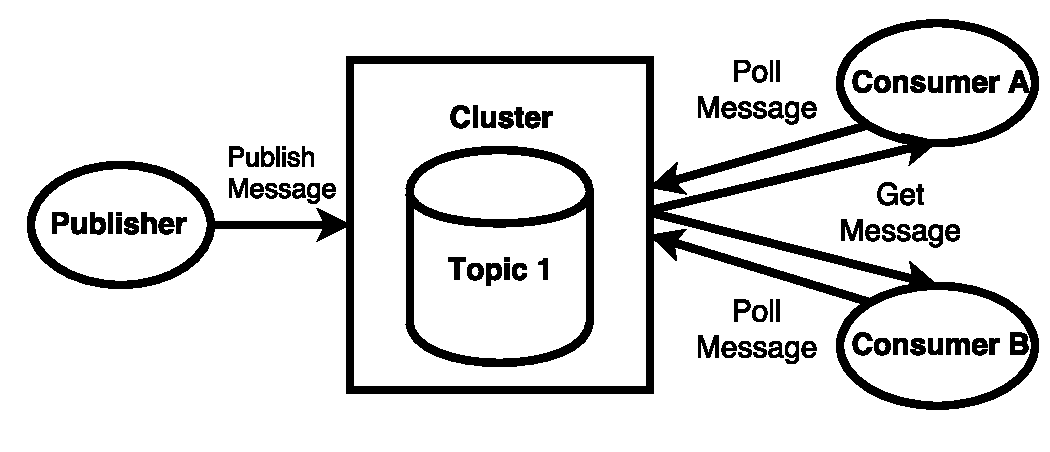
\includegraphics[scale=0.6]{figure/Kafka_topic_draw_Poll.pdf}
\pnote{* Poll verringert die Kopplung von Consumern und Producern}
\end{frame}

\begin{frame}
\frametitle{Kafka Topic}
\begin{itemize}
	\item Vereinigt klassischen Queue- und Topicansatz
	\item Multi-Subscribe ($0$ bis $n$ Consumer)		% Consumergroups - n Anzahl der Partitionen
	%\item Kein Push-System
	\pnote{* Enkopplung durch Pull!}
	\item Records in Topics werden persistent gehalten
	\pnote{* Record: Nachricht + Time}
	\item Topics benötigen eine Cleanup-Policy
		\begin{itemize}
			\item Retention-Time
			\pnote{* Retention-Time: nach gewisser Zeit löschen}
			\item Retention-Size
			\pnote{* Retention-Size: ab gewisser größe löschen}
			\item Log-Compaction
			\pnote{* Log-Compaction: hält von jeder message mit dem gleichen Key die neuste Nachricht. }
		\end{itemize}
	\item Guarantees
		\begin{itemize}
			\item Reihenfolge der Records wird eingehalten
			\pnote{Nachrichten in Reihenfolge im Log wie gesendet}
			\item Consumer sehen die Einträge wie im Log gespeichert
			\item N-1 Serverausfälle bei N Replikationen ohne Datenverluste
			\pnote{* Guarantees: Reihenfolgesicherung beim schreiben und lesen, Ausfall N-1 }
		\end{itemize}
\end{itemize}
\end{frame}

%% %%%%%%%%%%%%%%%%%%%%%%%%%%%%%%%% Partitionen %%%%%%%%%%%%%%%%%%%%%%%%%%%%%%%%
\begin{frame}
\frametitle{Partitionen}
\begin{itemize}
	\item Jedes Topic besteht aus $1..n$ Partitionen
	\item Eigenschaften von Partitionen
	\begin{itemize}
		\item Records sind geordnet
		\item Nicht-Veränderbare Sequenz von Records
		\item Records können nur angehängt werden
	\end{itemize}
	\item Records werden über \texttt{offset} identifiziert
	\item Records werden nach Cleanup-Policy entfernt
	\item Lesezugriff auf Records in Partitionen
	\begin{itemize}
		\item Aufsteigend sequentieller Zugriff ist Standard
		\item Wahlfreier Zugriff auf Records auch möglich
	\end{itemize}
\end{itemize}
\end{frame}

\begin{frame}
\frametitle{Partitionen}
	\centering
	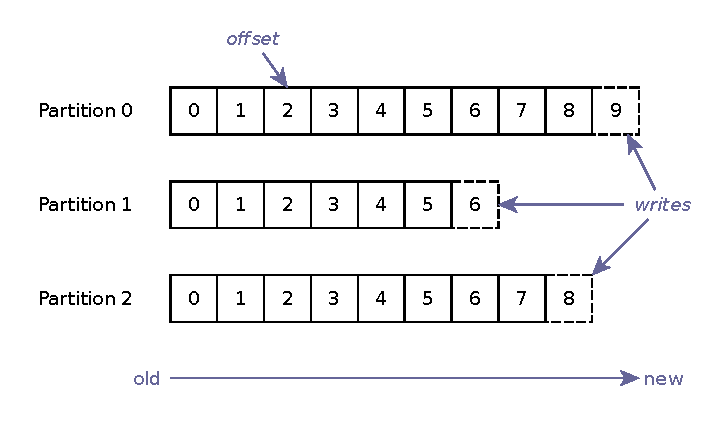
\includegraphics[scale=0.75]{figure/partitioned_log.pdf}
	
	\BottomRightText{\textit{Graphics based on}~\cite{Kafka}}
\end{frame}

\begin{frame}
\frametitle{Partitionen}
	\centering
	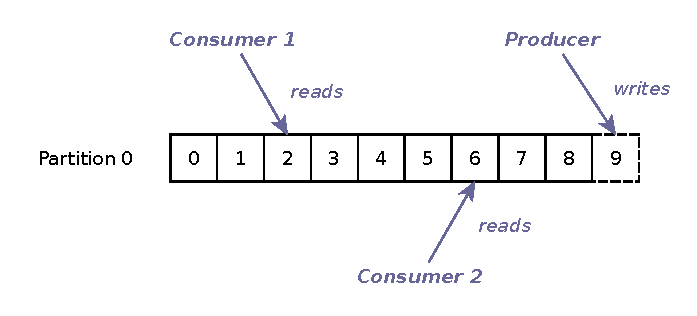
\includegraphics[scale=0.75]{figure/partition.pdf}
	
	\BottomRightText{\textit{Graphics based on}~\cite{Kafka}}
\end{frame}

\begin{frame}
\frametitle{Partitionen}
	Verteilung der Partitionen unterstützt
	\begin{itemize}
		\item Skalierung\\
			Topic kann durch Partitionen einfach auf mehrere Server verteilt werden.
		\item Parallele Verarbeitung
		\begin{itemize}
			\item Load Balancing
			\item Ordering Guarantees
			%Kafka is able to provide both ordering guarantees and load balancing over a pool of consumer processes
		\end{itemize}
	\end{itemize}
\end{frame}


%% %%%%%%%%%%%%%%%%%%%%%%%%%%%% Kafka Funktionen %%%%%%%%%%%%%%%%%%%%%%%%%%%%

\subsection{Eigenschaften von Kafka}
%% Messaging System
\begin{frame}
\frametitle{Kafka als Nachrichtensystem}
\centering
\begin{columns}[T] % contents are top vertically aligned
	\begin{column}[T]{.5\textwidth} 
		Consumer Groups
		\begin{itemize}
			\item Nachrichtenverarbeitung in Gruppen
			\item Mehrere Consumer werden in einer Gruppe organisiert
			\item Kombiniert Queueing und Publish-Subscribe
		\end{itemize}
	\end{column}
	\begin{column}[T]{.5\textwidth}
		\begin{figure}
		\centering
		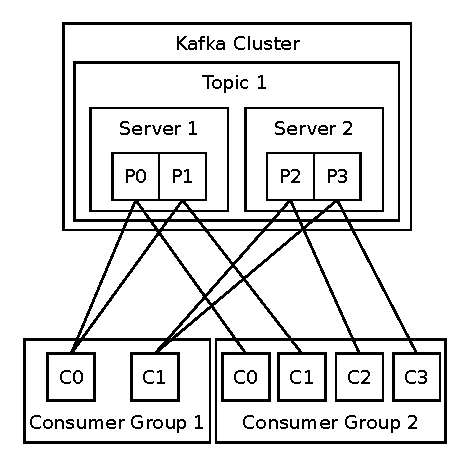
\includegraphics[scale=0.7]{figure/consumer_groups.pdf}
		\end{figure}
	\end{column}
\end{columns}

\BottomRightText{\textit{Graphics based on}~\cite{Kafka}}
\end{frame}

%\begin{frame}
%\frametitle{Parallelität?}
%\begin{itemize}
%	\item Ordnung 
%	\begin{itemize}
%		\item Gesichert für alle Consumer Groups
%	\end{itemize}
%	\item Lastverteilung
%		\begin{itemize}
%		\item Nachricht 1x pro Consumer Group verarbeitet
%	\end{itemize}
%\end{itemize}
%
%\end{frame}

%% Storage System
\begin{frame}
\frametitle{Kafka als Speichersystem}

\begin{block}{Kafka as a Storage System}
	"Kafka [is] a kind of special purpose distributed filesystem dedicated to high-performance, low-latency commit log storage, replication, and propagation." \cite{Kafka}
\end{block}


\begin{itemize}
	\item Entkopplung von Consumer und Producer sorgt für Speicherbedarf
	\item Daten werden immer persistent gehalten
	\begin{itemize}
		\item Kafka arbeitet somit \textit{nicht} In-Memory
	\end{itemize}
	\item Daten können repliziert werden
\end{itemize}
\end{frame}

\begin{frame}
\frametitle{Kafka für Stream Processing}

\begin{itemize}
	\item Anforderung: Streamverarbeitung in \textit{Echtzeit}!
	\item Ein Stream Processor
	\begin{itemize}
		\item nimmt kontinuierlich Daten aus einem \textit{Input} Topic,
		\item bearbeitet die Daten und
		\item schreibt kontinuierlich Daten in ein \textit{Output} Topic 
	\end{itemize}
\end{itemize}

\end{frame}


\begin{frame}
\frametitle{Kafka für Stream Processing - Stream API}

\begin{itemize}
	\item \texttt{Stream API} wird für nicht-triviales Stream Processing angeboten,
	z.B. zur Aggregation oder Joins von Streams. 
	\item \texttt{Stream API} unterstützt
	\begin{itemize}
		\item \textit{Exactly-once} Verarbeitung von Daten
		\item Statusbehaftete Operationen, wie Joins und Aggregationen über Bereiche
		\item Erneute Verarbeitung von Daten, wenn sich die Operation ändert
		\item \textit{One-record-at-a-time Processing}, um Verarbeitungs"-latenz im Milli"-sekunden"-bereich garantieren zu können
	\end{itemize}
\end{itemize}

%The streams API builds on the core primitives Kafka provides: it uses the producer and consumer APIs for input, uses Kafka for stateful storage, and uses the same group mechanism for fault tolerance among the stream processor instances.
\end{frame}

\subsection{Performance Analyse}
\begin{frame}{Performance Analyse}
\begin{figure}
	\centering
	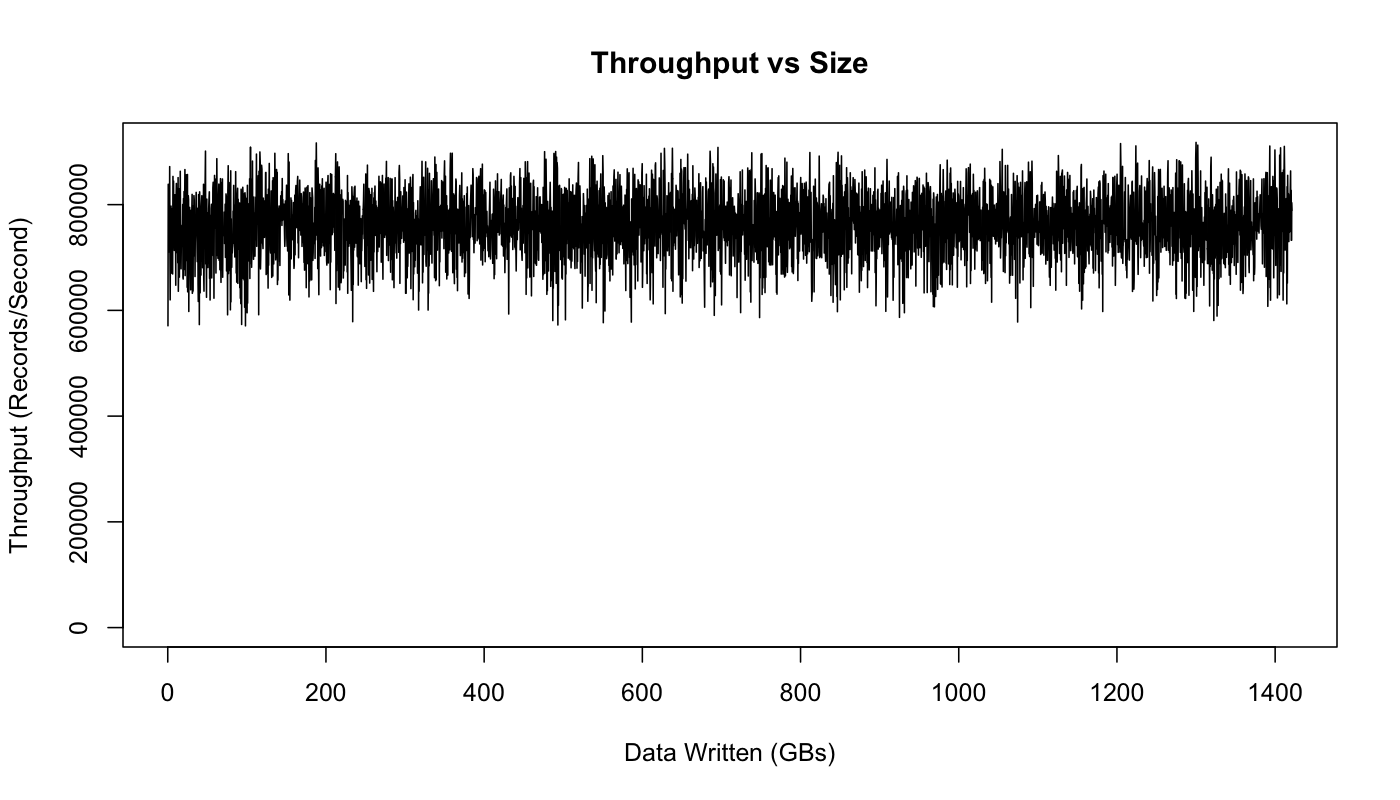
\includegraphics[scale=0.2]{figure/throughput_vs_size_0.png}
	\caption{Performance Analyse -- Durchsatz vs Datengröße~\cite{KafkaPerf}}
\end{figure}

	\pnote{- Don't fear the filesystem}
	\pnote{-- Weiterentwickluing der Festplatten und Optimierungsmöglichkeiten}	
	\pnote{-- Ensure linear write disk I/O -> können stark vom OS optimiert werden (read-ahead, write-behind)}
	\pnote{-- Batching together small bits of data}
	\pnote{}
	\pnote{- Kafka kann O(1)}
\end{frame}

\begin{frame}
\frametitle{Zusammenfassung}

% Wie verpacken?
%By combining storage and low-latency subscriptions, streaming applications can treat both past and future data the same way. That is a single application can process historical, stored data but rather than ending when it reaches the last record it can keep processing as future data arrives. This is a generalized notion of stream processing that subsumes batch processing as well as message-driven applications.

%Likewise for streaming data pipelines the combination of subscription to real-time events make it possible to use Kafka for very low-latency pipelines; but the ability to store data reliably make it possible to use it for critical data where the delivery of data must be guaranteed or for integration with offline systems that load data only periodically or may go down for extended periods of time for maintenance. The stream processing facilities make it possible to transform data as it arrives.

	\begin{itemize}
		\item Verteilte skalierbare Streaming Plattform.
		\item Stream Processing in Echtzeit möglich
		\item Persistente Datenhaltung erlaubt die Nutzung von Kafka für kritische Daten bzw. Anwendungen
		\item Sowohl Batch Processing als auch nachrichtengetriebene Anwendungen werden unterstützt
	\end{itemize}

\end{frame}

\begin{frame}
\frametitle{Fragen}
\begin{center}
\Large{Gibt es bisher Fragen?}
\end{center}
\end{frame}